\begin{figure}[!t]
    \centering
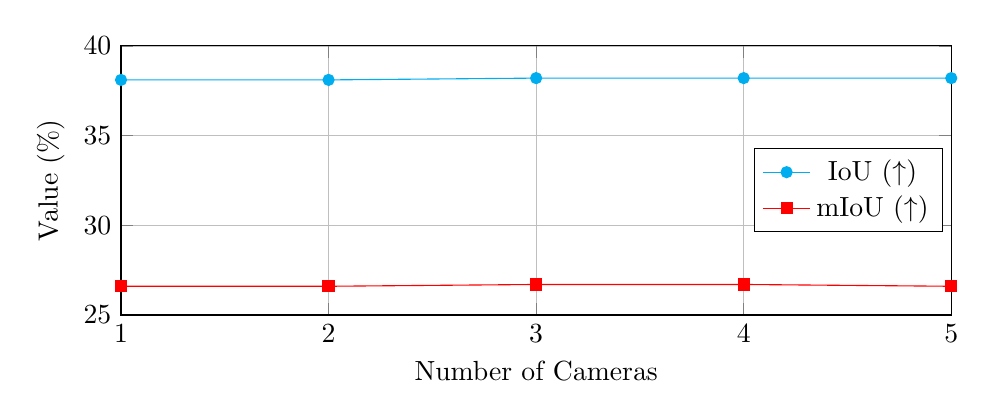
\begin{tikzpicture}
    \begin{axis}[
        width=\columnwidth,
        height=5cm,
        xlabel={Number of Cameras},
        ylabel={Value (\%)},
        xmin=1, xmax=5,
        ymin=25, ymax=40,
        xtick={1, 2, 3, 4, 5},
        xticklabels={1, 2, 3, 4, 5},
        ytick={25,30,35, 40},
        legend style={at={(0.99, 0.62)}},
        grid=both,
        grid style={line width=.1pt, draw=gray!10},
        major grid style={line width=.2pt, draw=gray!50},
    ]
        \addplot[
            color=cyan,
            mark=* ,
            mark options={solid, fill=cyan},
        ] coordinates {
            (1, 38.1)
            (2, 38.1)
            (3, 38.2)
            (4, 38.2)
            (5, 38.2)
        };
        \addlegendentry{IoU ($\uparrow$)}

        \addplot[
            color=red,
            mark=square*,
            mark options={solid, fill=red},
        ] coordinates {
            (1, 26.6)
            (2, 26.6)
            (3, 26.7)
            (4, 26.7)
            (5, 26.6)
        };
        \addlegendentry{mIoU ($\uparrow$)}
    \end{axis}
\end{tikzpicture}
    \caption{\textbf{Impact of the number of cameras on 3D semantic occupancy performance.} The architecture used is TPVFormer \cite{huang2023tpv}. Models are trained with varying numbers of cameras and evaluated on 3D IoU and mIoU using 20\% of Occ3d-nuScenes training and validation set.}
    \label{fig:num_cams_impact}
\end{figure}
